\section{In this problem you will use the delta(chi2) method to form a test statistic to discriminate between two types of events (let's call them type A and type B). See Lecture 17, slide 20 for the definition of this test statistic. You are given two large training sets of type A events and type B events. For each event two quantities have been measured: x (first column in the file) and y (second column), and there are 10,000 events in each training set. Use these training sets to define a delta(chi2) statistic analogous to what is shown on the slide referred to above. You are also given two testing sets of type A and type B events. Apply your delta(chi2) statistic to each testing set and plot the distributions of the test statistic for each type of events on the same plot. For a given event with x=2.5, y=-0.5, what fraction of type A events have a higher value of this test statistic? What fraction of type B events have a higher value? Given your results, can you calculate the probability that this particular event is of type A?}


\begin{itemize}
    \item Here's that plot (see code for how it was made):
    \begin{center}
        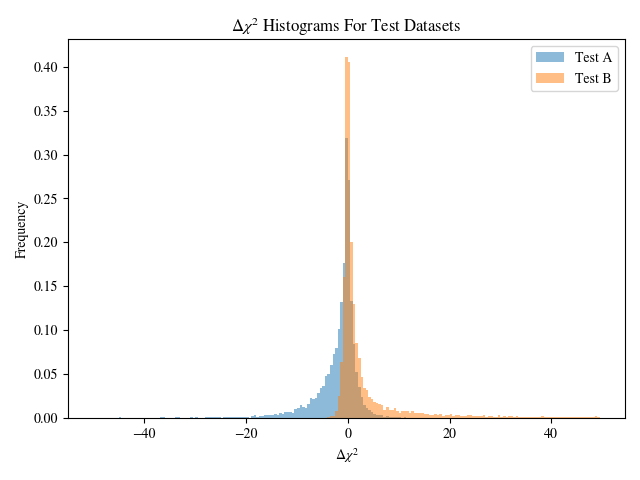
\includegraphics[width=0.7\textwidth]{q3.png}
    \end{center}

    \item For a given event with x=2.5, y=-0.5, what fraction of type A events have a higher value of this test statistic? What fraction of type B events have a higher value?
    
    $$f_A = 0.0823, f_B = 0.3099 \text{ (see code for calculation details)}.$$

    \item Given your results, can you calculate the probability that this particular event is of type A?

    No, since we don't know how likely we are to sample from type A vs type B -- e.g. if you have a 10\% chance of seeing this event in a sample of all As, and A happens once a day, and you have 1\% chance of seeing that in a sample of all Bs but B happens once a second, then if you see a random event (could be type A or B),  it's more likely for the event you saw to be a B even though you have a higher $f_A$.

\end{itemize}
